\section{Sentiment-Aspect-Region Model}
\label{sec:model}
We first present our objectives to build the
unified sentiment-aspect-region model.
To achieve the objectives, we present several intuitions
based on which we build our model.
We then describe the details of the model,
and propose a parameter estimation method.

\subsection{Intuitions}
\label{sec:motiv}
%We first introduce some notions that are used in
%explaining our objectives. There are three types of
%latent factors that are not observable in a geotagged review corpus, but
%are important for user preference analysis. They
%are topical-region, topical-aspect and sentiment.
%A topical-region represents a geographical area in which
%users do similar things (such as dining).
%%write region-specific words on their reviews.
%It comprises two components: geo-location and semantics.
%The geo-location component is usually modeled as a
%Gaussian distribution over
%POIs \cite{Yin:2011,YuanW4:2013}.
%The semantic component is modeled as a multinomial
%distribution over words \cite{Geofolk:2010}.
%Example topical-regions include shopping areas, education areas,
%streets of special snacks, etc.
%Topical-aspects are the aspects of POIs that
%are commented by users, such as environment, taste,
%price, etc. Sentiments are user's opinions over
%topical-aspects (e.g., positive, negative or neutral).
%%\KZ{Can sentiments be casted over regions? e.g., I hate
%%Clarke Quay!}
%Topical-aspects
%and sentiments can be modeled jointly \cite{JoASUM:2011}.

In this paper,
we aim at building a model that is able to 1) extract
latent variables, i.e., topical-aspect, sentiment,
and topical-region from the review
data; 2) capture the interdependencies among
category, POI, user, words and the three latent
variables; and 3) discover user's topical-region and
topical-aspect preferences.
To achieve these objectives,
we exploit the following intuitions in designing our model:

\textbf{Intuition 1}: A user visits POIs in a topical-region
because the region is geographically convenient to the user
(e.g., close to her activity areas) and its topics (e.g., shopping
street, education area, etc.) satisfy
the user's interest. Each user has her own preferences on the
topical-regions.
%We use a topical-region
%variable $r$ to model the mixture of topic and geographic
%information,
%i.e., each region exactly covers POIs of similar
%topic distribution and close in spatial.

\textbf{Intuition 2}: A user rates highly of a POI because
she likes some aspects of the POI. Such preferences might be
indicated in her review.
%i.e., user has preferences on some aspects of the POI.
Some users like to check the price range of a restaurant first while
others might be more concerned with the environment. Moreover, POIs in different
categories may have different aspects of interest.
%For
%instance, a traveler might care more about the environment
%of a hotel, while a hungry would-be diner might be more interested in
%the waiting time of a restaurant.

\textbf{Intuition 3}:
A user decides to visit a POI in a region
by considering the category, category-aware topical-aspects of the POI and
the distance to it. For example, users may visit POIs of the
restaurant category with good environment,
but she may first consider the restaurants nearby.
%to walk around a nearby shopping street.
%and visit
%POIs without being particular about the category.

\textbf{Intuition 4}: When a user writes a review on a POI, she
will use words for both the aspects of the POI and
her sentiments about the aspects.
The user may also use words for the topical-region of the POI.
For example, a review on a shop in Times Square may say:
``This shop offers best prices in Times Square.'' The reviewer
uses ``price'' for {\em aspect}, ``best'' for {\em sentiment}
and ``Times Square'' for {\em region}. %to construct the review.
%Moreover, each sentence in the review normally
%corresponds to exactly one aspect and
%users only associate one sentiment on each aspect. As a result,
%the words co-occurs in the same sentences are more likely to be correlated to
%the same aspect and sentiment.

\subsection{Model Description}
We first define the notations
to be used in the proposed model. Let $D$ be the set of user reviews,
and $U$ be the set of users. For each review, we denote the
number of its sentences by $M$ and number of words in each
sentence by $N$. In our model, a location has two attributes:
identifier and coordinates. We use $l$ to represent a location identifier
and $\boldsymbol{cd}_l$ to denote its corresponding coordinates.
Here $\boldsymbol{cd}_l$ is a latitude and longitude pair. We denote
the topical-aspect, sentiment and topical-region by $a$, $s$,
and $r$, respectively. The notations
used in this paper are listed in \tabref{tab:notation}.
Following the intuitions discussed in \secref{sec:motiv}, we
proceed to present our model.

\begin{table}[th]
\centering
%\scriptsize
\caption{Description of Symbols}
\begin{tabular}{l|l}
\hline
 Symbol & Description\\
\hline
$u$, $U$ & individual user and the set of users\\
\hline
$l$, $L$ & individual POI and the set of POIs  \\
\hline
$c$ & category  \\
\hline
$r$ & topical-region  \\
\hline
$a$, $s$ & topical-aspect and sentiment \\
\hline
$d$, $D$ & single review and the set of reviews \\
\hline
$M$ & the number of sentences in a review \\
\hline
$w$, $N$ & single word and the number of words in a sentence \\
\hline
\end{tabular}
\label{tab:notation}
\end{table}

Based on \textbf{Intuitions 1\&2}, we model the user
topical-region preferences and topical-aspect preferences
as multinomial distributions $p(r|u)$ and $p(a|u,c)$, respectively.

Based on \textbf{Intuition 3}, a user chooses a POI to visit
by considering both the category and the distance. We
define the probability of visiting a POI $l$ given
category $c$ and region $r$ proportional to $p(l|c)\cdot p(l|r)$.
Here $p(l|c)$ is the probability of selecting POI $l$ from
the category $c$; $p(l|r)$ is a the probability
of selecting POI $l$ in region $r$ by considering
the distance from $l$ to $r$. After normalization, we have the
definition $p(l|c,r)=\frac{p(l|c)p(l|r)}{\sum_{l'}{p(l'|c)p(l'|r)}}$.
%The denominator is used to normalize
%the $p(l|c)p(l|r)$ over all POIs.
To model the spatial distance, we use a
Gaussian mixture model, i.e.,
$p(l|r)\sim N(\boldsymbol{\mu}_r, \boldsymbol{\Sigma}_r)$, where
$\boldsymbol{\mu}_r$ is the center of region $r$ and
$\boldsymbol{\Sigma}_r$ is the co-variance matrix which depicts the
area of region $r$.
To model the membership of a POI to a category, we use a uniform
distribution for $p(l|c)$.
%$\kappa$ is tunable parameter used
%for balance the weights of generating POI from category and region.
%Note that $p(l|r)$ is a continuous distribution while $p(l|c)$ is
%a discrete distribution.
%To multiply the two distributions,
%we adopt the coordinate transformation approach for the Gaussian
%distribution that is proposed in Yuan et al.\cite{YuanW4:2013}.

Based on \textbf{Intuition 4},
we model the relationships among words, topical-aspects,
sentiments and topical-regions by
$p(w|a,s,r)=\lambda p(w|a,s)+(1-\lambda) p(w|r)$, where
$a$, $s$, $r$ are topical-aspect, sentiment and
topical-region, respectively.
Here $p(w|a,s)$ is the probability that the users write
word $w$ when they have sentiment $s$ on aspect $a$;
$p(w|r)$ is the probability that the users use word
$w$ to describe region $r$; parameter
$\lambda$ is used to balance the portion of
words drawn from topical-aspect, sentiment or topical-region.
We model $p(w|a,s)$ instead of $p(w|a)$ and $p(w|s)$
because aspects and sentiments are closely coupled,
and modeling by $p(w|a)$ and $p(w|s)$
needs an additional tuning parameter.
Similar to proposals of sentence level sentiment analysis
\cite{TitovMGLDA:2008,TitovMAS:2008, JoASUM:2011},
we assume each sentence expresses opinions on exactly one topical-aspect
and each topical-aspect is associated to a positive, negative or neutral sentiment.

\begin{figure}[th]
\centering
\epsfig{file=fig/modeldraft.eps,width=0.65\columnwidth}
\caption{Sentiment-Aspect-Region Model (SAR)}
\label{fig:model}
\end{figure}

In summary, the graphical representation of our model
is shown in \figref{fig:model} and
the generative process of the
reviews written by user $u$ is described as follows:
\begin{itemize}
\item For each review $d\in D_u$, where $D_u$ is the set of reviews written by user $u$.
    \begin{itemize}
    \item Draw topical region $r\sim p(r|u)$
    \item Draw category $c\sim p(c|u)$
    \item Draw location $l\sim p(l|c,r)=\frac{p(l|r)p(l|c)}{\sum_{l'}{p(l'|c)p(l'|r)}}$, where $p(l|r)\sim N(\boldsymbol{\mu}_r,\boldsymbol{\Sigma}_r)$
    \item For each sentence in review $d$
        \begin{itemize}
        \item Draw aspect $a\sim p(a|u,c)$
        \item Draw sentiment $s\sim p(s|a,l)$
        \item For each word position in the sentence
            \begin{itemize}
            \item Draw word $w\sim p(w|a,s,r)={\lambda}p(w|a,s)+(1-\lambda)p(w|r)$
            \end{itemize}
        \end{itemize}
    \end{itemize}
\end{itemize}

In the model, $p(l|c)$ and
$p(c|u)$ can be estimated directly from a given corpus. The
other distribution parameters need to be inferred.
We first present how to estimate $p(l|c)$ and
$p(c|u)$, and then show the inference algorithm for
the remaining distributions in \secref{sec:infer}.

As described in \textbf{Intuition 3},
a POI $l$ is generated from both category
and region. Since POI $l$ and category $c$ are
observable variables, we simply compute $p(l|c)$
by \equref{eq:plc}.
\begin{equation}
p(l|c)=\frac{I(l,c)}{\#\; of\; POIs\; in\; c}
\label{eq:plc}
\end{equation}
\begin{equation}
I(l,c)=
\begin{cases}
1 & l\in c \\
0 & otherwise \\
\end{cases}
\end{equation}

Similarly, we compute the category preferences of each user, i.e., $p(c|u)$,
directly from the corpus. To handle the overfitting problem,
we apply the additive smoothing technique. After smoothing, even though a user did
not a visit some category of POIs, the probability of
visiting that category still has a small value. The computation of $p(c|u)$ is shown in
\equref{eq:pcu}.
\begin{equation}
p(c|u)=\frac{n_c+\alpha}{N+{\alpha}C},
\label{eq:pcu}
\end{equation}
where $n_c$ is the number of reviews of POIs in category $c$ that user $u$
writes; $N$ is the total number of reviews on POIs in $c$; $C$
is the total number of categories; $\alpha$  is the smoothing
parameter which is usually set to a value smaller than 1. In this paper,
we set $\alpha=0.1$.

\subsection{Inference Algorithm}
\label{sec:infer}
To infer the parameters of the model, we
use the expectation-maximization (EM) approach.
In this section,
we present the computation of the corpus
likelihood, the two-step EM algorithm
used to infer our parameters, and
initialization of the EM algorithm.

\subsubsection{Likelihood Computation}
Our model has several levels, i.e., word level,
sentence level, and document level. The latent variables
are on two levels. Region $r$ is at document level while
aspect $a$ and sentiment $s$ are at sentence level.
This multi-level structure poses challenges to the estimation of
the log-likelihood. According to the generative
process, we have the likelihood of the corpus $D$:
\begin{equation}
p(D;\Phi)=\prod_{d}^{D}{p(u_d)\sum_{r}^{R}{p(r|u_d)}p(l_d,\mathbf{w}_d|r,u_d)}
\label{eq:likeli1}
\end{equation}
\begin{equation}
p(l_d,\mathbf{w}_d|r,u_d)=p(c_{l_d}|u_d)p(l_d|r,c_{l_d})\prod_{i}^{M}{p(\mathbf{w}_{d,i}|c_{l_d},r,u_d,l_d)}
\label{eq:likeli2}
\end{equation}
\begin{equation}
\begin{split}
&p(\mathbf{w}_{d,i}|c_{l_d},r,u_d,l_d) \\
&=\sum_{a,s}{p(a|c_{l_d},u_d)p(s|a,l_d)\prod_{j}^{N}{p(w_{d,i,j}|a,s,r)}}
\end{split}
\label{eq:likeli3}
\end{equation}
In \equref{eq:likeli1}, $\Phi$ is the set of parameters in the model,
i.e., $p(r|u)$, $p(a|c,u)$,$p(l|r)$,$p(s|a,l)$,$p(w|a,s)$,
$p(w|r)$,$\boldsymbol{\mu}_r$ and $\boldsymbol{\Sigma}_r$.
Variables $u_d$,$l_d$,$\mathbf{w}_d$ are the user, location and
words of review $d$, respectively. Variable $\mathbf{w}_{d,i}$
represents the set of words in sentence $i$ of review $d$
while $w_{d,i,j}$ is the $j^{th}$ word in sentence
$i$ of review $d$. Taking logarithm of
$p(D;\Phi)$ leads to a summation inside the logarithm:
\begin{equation}
L=\sum_{d}{\log{p(u_d)}+\log{\sum_{r}{p(r|u_d)p(l_d,\mathbf{w}_d|r,u_d)}}}
\label{eq:loglikeli}
\end{equation}
Since this likelihood cannot be estimated directly,
we adopt Jessen's
inequality to the log-likelihood, and estimate the
lower bound of the likelihood and the parameters
in an iterative manner.

\subsubsection{Expectation-Maximization}
Due to the aforementioned difficulty of computing
log-likelihood directly,
we apply Expectation-Maximization (EM)
algorithm to estimate the model parameters.

In \textbf{E-step}, we compute the expectation
of latent variables given the observed data.
By applying Jessen's inequality to \equref{eq:loglikeli},
we get the lower bound of the likelihood as:
\begin{equation}
\begin{split}
L_{LB}=&\sum_{d}{\log{p(u_d)}}\\
+&\sum_{d,r}{p(r|d)(\log{p(r|u_d)}+\log{p(l_d,\mathbf{w}_d|r,u_d)})}
\end{split}
\label{eq:loglikeli1}
\end{equation}
As shown in \equref{eq:loglikeli1},
we need to estimate $p(r|d)$ to compute the full likelihood.
We apply Bayes rule, and obtain the update
function of the posterior distribution as
\begin{equation}
p(r|d)=\frac{p(r,d)}{\sum_{r}{p(r,d)}}
\label{eq:prd}
\end{equation}
\begin{equation}
p(r,d)=p(u_d)p(r|u_d)p(l_d,\mathbf{w}_d|r,u_d)
\label{eq:prdjoint}
\end{equation}
In \equref{eq:prdjoint},
$p(l_d,\mathbf{w}_d|r,u_d)$ is computed by \equref{eq:likeli2}, and
$p(u_d)$ appears both in the numerator and the denominator,
and thus is not necessary to estimate.

In \textbf{M-step}, by maximizing the lower bound of likelihood,
we can obtain the update function of parameters at document level
that are related to topical region $r$ as below.
\begin{equation}
p(r|u)=\frac{\sum_{d\in D_u}{p(r|d)}}{\sum_{r}{\sum_{d\in D_u}{p(r|d)}}}
\label{eq:pru}
\end{equation}
%\begin{equation}
%\boldsymbol{\mu}_r=\frac{\sum_{d}{p(r|d)\cdot \boldsymbol{cd}_{l_d}}}{\sum_{d}{p(r|d)}}
%\label{eq:mu}
%\end{equation}
%\begin{equation}
%\boldsymbol{\Sigma}_r=\frac{\sum_{d}{p(r|d)\cdot (\boldsymbol{cd}_{l_d}-\boldsymbol{\mu}_r)^T(\boldsymbol{cd}_{l_d}-\boldsymbol{\mu}_r)}}{\sum_{d}{p(r|d)}}
%\label{eq:sigma}
%\end{equation}

However, we cannot obtain a close form solution for $\boldsymbol{\mu}_r$ and
$\boldsymbol{\Sigma}_r$ due to the normalization term. We adopt a gradient method
to obtain the update value of $\boldsymbol{\mu}_r$ and $\boldsymbol{\Sigma}_r$ in M-step.
Specifically, we use the BFGS quasi-Newton method \cite{Kurashima:2013,Liu:1989}.
In the gradient method, we compute the gradient of $\boldsymbol{\mu}_r$ and
$\boldsymbol{\Sigma}_r$ as follows:
\begin{equation}
\frac{\partial L_{LB}}{\partial \boldsymbol{\mu}_r}=
\sum_d{p(r|d)\boldsymbol{\Sigma}_r^{-1}\left(\frac{\sum_{l'}{q(l')(\boldsymbol{cd}_{l'}-\boldsymbol{\mu}_r)}}{\sum_{l'}{q(l')}}-
(\boldsymbol{cd}_{l_d}-\boldsymbol{\mu}_r)\right)}
\label{eq:gmu}
\end{equation}
\begin{equation}
\frac{\partial L_{LB}}{\partial \boldsymbol{\Sigma}_r}=\sum_d{p(r|d)(\frac{\sum_{l'}{q(l')g(l', r)}}{\sum_{l'}{q(l')}}-g(l_d, r))}
\label{eq:gsigma},
\end{equation}
%\begin{equation}
%g(l, r)=-\frac{1}{2}\boldsymbol{\Sigma}_r^{-1}+\frac{1}{2}\boldsymbol{\Sigma}_r^{-1}(\boldsymbol{cd}_{l}-\mu_r)(\boldsymbol{cd}_{l}-\mu_r)^T\boldsymbol{\Sigma}_r^{-1}
%\end{equation}
where $q(l')=p(l'|c_l)p(l'|r)$ and $\boldsymbol{cd}_{l}$ denotes the coordinates of POI $l$.
The function $g(l, r)$ in \equref{eq:gsigma} is the gradient of the Gaussian distribution for region $r$
w.r.t. $\boldsymbol{\Sigma}_r$ at point $l$.

Since sentiment and aspect are at the sentence level, we
cannot compute $\log p(l_d,\mathbf{w}_d|r,u_d)$
in \equref{eq:loglikeli1} using $p(r|d)$. 
Thus, we propose a second level of EM iterations.
Specifically, we introduce a new latent variable to estimate parameters related to
aspect and sentiment. Specifically, we use $\phi_{a,s,r,d_i}$ to identify
the probability that the $i^{th}$ sentence in a review $d$ from
region $r$ is assigned with aspect $a$ and sentiment $s$.
we use $\phi_{a,s,r,d_i}$ and $p(r|d)$ to compute the update
function of $p(a|c,u)$, $p(s|l,a)$,
$p(w|a,s)$, and $p(w|r)$.

Denote by $n(w,d_i)$ the number of occurrences of word $w$ in sentence $i$
of review $d$. We estimate $\phi_{a,s,r,d_i}$ as:
\begin{equation}
\phi_{a,s,r,d_i}=\frac{p(a,s,r,d_i)}{\sum_{a,s}{p(a,s,r,d_i)}}
\label{eq:pasrdi}
\end{equation}
\begin{equation}
\begin{split}
p(a,s,r,d_i)=p(u_d)p(r|u_d)p(c_{l_d}|u_d,r)p(l_d|r,c_{l_d})\\
p(a|c_{l_d},u_d)p(s|a,l_d)\prod_{w}{p(w|a,s,r)^{n(w,d_i)}}
\end{split}
\end{equation}

By maximizing the lower bound of the likelihood, we
obtain the update function of the rest parameters:
\begin{equation}
p(a|u,c)=\frac{\sum_{d\in D_u}{\sum_{r}{p(r|d)\sum_{i}{\sum_{s}{\phi_{a,s,r,d_i}}}}}}{\sum_{a'}{\sum_{d\in D_u}{\sum_{r}{p(r|d)\sum_{i}{\sum_{s}{\phi_{a',s,r,d_i}}}}}}}
\label{eq:pacu}
\end{equation}
\begin{equation}
p(s|l,a)=\frac{\sum_{d\in D_l}{\sum_{r}{p(r|d)\sum_{i}{\sum_{s}{\phi_{a,s,r,d_i}}}}}}{\sum_{s'}{\sum_{d\in D_l}{\sum_{r}{p(r|d)\sum_{i}{\sum_{s}{\phi_{a,s',r,d_i}}}}}}}
\label{eq:psal}
\end{equation}
\begin{equation}
p(w|s,a)=\frac{\sum_{d}{\sum_{r}{p(r|d)\sum_{i}{\phi_{a,s,r,d_i}n(w,d_i)}}}}{\sum_{w'}{\sum_{d}{\sum_{r}{p(r|d)\sum_{i}{\phi_{a,s,r,d_i}n(w',d_i)}}}}}
\label{eq:pwsa}
\end{equation}
\begin{equation}
p(w|r)=\frac{\sum_{d}{p(r|d)\sum_{i}{\sum_{a}{\sum_{s}{\phi_{a,s,r,d_i}n(w,d_i)}}}}}{\sum_{w'}{\sum_{d}{p(r|d)\sum_{i}{\sum_{a}{\sum_{s}{\phi_{a,s,r,d_i}n(w',d_i)}}}}}},
\label{eq:pwr}
\end{equation}
where $D_u$ is the set of reviews written by user $u$ and $D_l$
is the set of reviews for POI $l$.

\subsubsection{Initialization of EM Algorithm}
EM algorithm can only guarantee to find a local optima.
Different initializations may lead to different results.
In this section, we present our methods for initializing the assignment of
aspect, sentiment and region.

\textbf{Aspect} is extracted from sentence level in our model.
We initialize the aspect by a clustering process on
sentences. Each sentence is represented as a vector of words.
Given the number of aspects, we use K-means clustering
algorithm to assign each sentence an aspect.
We then initialize $p(w|a)$ by the probability that word
$w$ appears in sentences carrying aspect $a$.

\textbf{Sentiment} has 3 possible values in this paper:
positive, negative and neutral.
In order to know the polarity of each sentiment, we need some prior
knowledge. We use the same predefined set of sentiment seed words
as in Jo's proposal \cite{JoASUM:2011}. Moreover, we apply a syntactic parser to
extract negation of the sentiment words such as ``not good'' and
use a special word ``not\_good'' to represent the phrase ``not good''
in our vocabulary. For each word in the seed word set, we assign
a probability ($p(w|s)$) of 1 to its polarity and 0 to the other
two polarities. For words not in the seed word set, we assign an
equal probability for each polarity. We then use $p(w|a)p(w|s)$
to approximate $p(w|a,s)$.

\textbf{Region} is initialized by a K-means clustering
algorithm based on the coordinates (latitude and longitude).
The clustering algorithm partitions POIs to different
regions. Then for each region r, we compute $\boldsymbol{\mu}_r$
and $\boldsymbol{\Sigma}_r$ using a regression
over the POIs in the region.
We compute $p(w|r)$ by the distribution of
words in the reviews for POIs in region $r$ and $p(r|u)$ by the
portion of reviews that user $u$ writes in region $r$.

For other parameters: $p(a|c,u)$ and $p(s|a,l)$, we initialize
them by using the assignment of aspect and sentiment to a sentence
(We assign sentiment to a sentence by voting from sentiment seed words
extracted from the sentence). Specifically, $p(a|c,u)$ is proportional to the
number of sentences that are assigned to $a$ and that belong to a review
written by $u$ from category $c$; $p(s|a,l)$ is proportional to
the number of sentences that belong to location $l$ and
are assigned to sentiment $s$ and aspect $a$ at the same time.

\subsubsection{Efficiency Analysis}
Let the number of sentiment be 3 and we treat it as
constant. In E-step,
the computation of the expectation of latent variables in \equref{eq:prd}
and the variables $\phi_{a,s,r,d_i}$ in \equref{eq:pwr}
needs $O(|D|MNRA)=O(WRA)$, where $W$ is the number of words in the reviews of all
users' in training set,
$R$ is the number of regions and $A$ is the number of aspects.
In M-step, the cost for updating \equref{eq:pacu} to (\ref{eq:pwr})
is $O(UA+LA+VA+VR)$,
where $U,L,V$ are the number of users, POIs and unique words, respectively.
To update $\boldsymbol{\mu}$ and $\boldsymbol{\Sigma}$, we perform a
quasi-Newton method. Since each $\boldsymbol{\mu}_r$ and $\boldsymbol{\Sigma}_r$
are two dimensional vector and $2\times2$ matrix, respectively. The computation cost of matrix operation
can be treated as constant. Let $D$ be the number of reviews, the cost of
computing gradient in \equref{eq:gmu} and (\ref{eq:gsigma})
is $D+L$.
Therefore, the complexity of quasi-Newton is $O(I_qR(D+L))$, where $I_q$
is the number of iterations of quasi-Newton.
In summary, the total complexity of the learning
algorithm with $I$ iterations is $O(I(WRA+I_qR(D+L)+UA+LA+VA+VR))$.
Since $WRA\gg (UA+LA+VA+VR)$, we simplify the cost as $O(I(WRA+I_qR(D+L)))$.
%The training complexity is high, but
%fortunately, the training process can be done offline,
We can parallelize the computation
of both E-step and M-step. In E-step, since
the computation of $p(r|d)$ on each document is independent to others, we can compute $p(r|d)$
of each document in parallel. In M-step, the update of \equref{eq:pacu} to (\ref{eq:pwr}) and
the quasi-Newton iterations can also be
parallelized in the similar way as $p(r|d)$. Therefore, the algorithm can be fully parallelized.

\section{Applications}
\label{sec:app}
%Our model can be applied to POI recommendation and user recommendation.
%We show in detail how to use the estimated parameters for recommendation.
We present three applications of our model, namely POI recommendation,
user recommendation, and aspect satisfaction analysis in regions. In POI recommendation,
we provide a way to explain the reason of recommending a POI and
propose an efficient online recommendation algorithm.
% region-aware users' satisfaction estimations.

\subsection{POI recommendation}
\label{sec:model-poirec}
%Most of the existing proposals for POI recommendation are
%based on collaborative filtering.
%Ye et al. \cite{YeGeoSocial:2011} propose a fusion framework to
%combine user-based, friend-based and geo-based collaborative
%filtering. In the geographic model, the probability of transporting
%from one POI to another is drawn from a power law distribution over
%the distances between the two POIs. The probability of a user
%visiting a POI is given by considering the distances between the
%POI and the POIs visited by the user. Yuan et al.
%\cite{YuanPOI:2013} propose a time-aware model
%for recommendation where check-ins
%are divided into different groups by different time segments to
%model user interests by time. Yang et al. \cite{YangSenti:2013}
%propose a sentiment-enhanced location recommendation
%system. They combine both check-ins and
%the overall sentiment on each location
%and apply probabilistic matrix factorization for recommendation.
%Different from these proposals, our model recommends POIs based
%on user topical-aspect preferences, topical-region preferences
%and the aspect-level sentiment of the POIs.

We apply our model to two POI recommendation tasks
and propose an efficient online recommendation algorithm.
The two recommendation tasks are \emph{All-Category Recommendation}
and \emph{Single-Category Recommendation}.

\subsubsection{All-Category Recommendation}
All-Category Recommendation is a task of
generating a rank list of POIs in any category
given a set of POIs and a user.
%When
%a user wants to visit a place without specifying the category,
%she needs recommendation from all of the categories.
The aforementioned proposals are all for all-category recommendation.
We calculate the
probability of $p(l,s_+|u)$, i.e., the probability of user
$u$ visits POI $l$ with positive sentiment, to score $l$ for $u$
as shown in \equref{eq:poiacr}.
\begin{equation}
\begin{split}
p(l,s_+|u)=&\sum_{r}{p(r|u)p(c_l|u)p(l|r,c_l)}\\
&\sum_{a}{p(a|u,c_l)p(s_+|a,l)}
\label{eq:poiacr}
\end{split}
\end{equation}
According to \equref{eq:poiacr}, we make the recommendation
by considering the matching between user preferences (i.e., $p(r|u)$,
$p(c_l|u)$ and $p(a|u,c_l)$) and the attributes of the POI
(i.e., $p(s_+|a,l)$ and $p(l|r,c_l)$).
%Only when the location satisfy the preference, i.e., the probabilities
%$p(s_+|a,l)$ and $p(l|r)$ are high for the user's preferred aspects $a$
%and region $r$, will $l$ be probably visited
%and satisfied by user $u$.
%In summary, our model considers aspect($p(a|u,c)$),
%sentiment($p(s_+|a,l)$) and region($p(r|u)p(l|r)$) when
%giving a recommendation.

This recommendation model enables us to explain why we recommend
a POI to a user. We consider two factors: aspect and region.
First, we rank the aspects by $p(s_+|a,l)p(a|u,c_l)$ to reveal
which aspects match the user's preferences.
Second, we rank the regions by $p(r|u)p(l|r)$ to reveal which regions
contribute more to the recommendation. Finally, we choose top several
aspects and regions for explanation.

\subsubsection{Single-Category Recommendation}
Single-Category Recommendation aims at
ranking POIs given a user and
a specific category (e.g., restaurants).
It is a typical scenario for POI recommendation
although it has not been covered in previous work.
We compute $p(l,s_+|u,c)$ as shown in \equref{eq:poiscr}.
Compared to all-category recommendation, we fix the category
i.e., remove $p(c|u)$ from \equref{eq:poiacr}.
All locations that are not in $c$ will not be
considered in this scenario.
\begin{equation}
\begin{split}
p(l,s_+|u,c)=&\sum_{r}{p(r|u)p(l|r,c)}\\
&\sum_{a}{p(a|u,c)p(s_+|a,l)}
\label{eq:poiscr}
\end{split}
\end{equation}
We can also offer explanation for the single-category recommendation
by following similar method as we employ for the all-category recommendation.

\subsubsection{Efficient algorithm for Top-N Online Recommendation}
Time efficiency is an essential part of online recommendation. A straightforward
method of making recommendation is to compute the recommendation score as \equref{eq:poiacr}
or \equref{eq:poiscr}.
This method requires traversing all the regions which is highly time consuming.
Another choice is the threshold algorithm \cite{FaginTA:2001}
that may save the computation for some POIs.
However, in our applications, the
number of attributes (i.e., regions and aspects) is large, and thus it is expensive
to compute the recommendation score even for a single POI.
The threshold algorithm cannot help with this, either.
We propose an optimized top-N items recommendation algorithm that significantly
reduces the time cost. As to be shown in the experiment,
our algorithm is faster than the threshold algorithm
in the top-N POI recommendation using our model. Our algorithm
can be applied to all or single-category POI recommendation. % as well as user recommendation.
We use all-category POI recommendation (\equref{eq:poiacr})
as an example to explain the algorithm.

Our algorithm is based on two observations:
1) A user only prefers a small number of regions;
and 2) POIs in the center of the
region are more likely to be recommended. These two observations indicate that only when
a user prefers a region and the POI is near the center of the region, will the score
$p(r|u)p(l|r,c_l)$
contribute significantly to the recommendation score.
Therefore, after we have computed the most possible regions for a POI,
it may not be necessary to compute the remaining regions.
We design a branch and bound algorithm as shown in Algorithm \ref{oprec}
to prune the search space of the regions.
Our algorithm contains two steps: \emph{initialization} and \emph{pruning}.
%By using the second observation, we can produce a
%good initial top-N list.

%Consider the POI recommendation mentioned in \equref{eq:poiacr}.
In the \emph{initialization} step (line 2),
we find $N$ candidate POIs that are potentially
good for recommendation.
Specifically, we pick top $K$ regions which
cover most of the user's regional preferences
(i.e., $\sum_{i=1}^{K}{p(r_i|u)}>0.9$) with smallest $K$ (line 21).
If $K$ is larger than $N$, we pick at most $N$ regions
to ensure that we can select at least one candidate from each region.
In each of the top $K$ region, we choose top $\ceil*{\frac{N}{K}}$
POIs w.r.t. $p(l|r)$ as candidates.

In the \emph{pruning} step (line 9-10),
we check whether we can avoid traversing unnecessary regions for each POI.
%we check whether there is a POI that
%has a larger recommendation score than the smallest one in the candidate set.
%To compute the recommendation score, we need to traverse all regions
%to sum up $p(r|u)p(l|r,c_l)$ for each POI in the straightforward method.
We traverse the regions according to
the descending order of $p(l|r,c_l)$ for POI $l$. Suppose we have traversed regions
$\{r_1,...,r_{i-1}\}$. The partial score we have computed for the traversed regions is
\[PScore=\sum_{j=1}^{i-1}{p(r_j|u)p(l|r_j,c_l)}.\]
When we explore the i-th region, we compute the upper bound of
recommendation score for the POI as:
\begin{equation}
\label{eq:bound}
Bound^{(i)}(l)=PScore+(1-\sum_{j=1}^{i-1}{p(r_j|u)})p(l|r_i,c_l).
\end{equation}
%and $\sum_a{p(s_+|a,l)p(a|u,c_l)}=1$

Because we check the regions in the descending
order of $p(l|r,c_l)$, the actual value of $p(l|r,c_l)$
for the remaining regions should be less than the one
for the current region, i.e., $p(l|r_i,c_l)$.
Therefore, we have a partial recommendation
score for the rest of the regions, which is at most
\[(1-\sum_{j=1}^{i-1}{p(r_j|u)})p(l|r_i,c_l),\]
where
$1-\sum_{j=1}^{i-1}{{p(r_j|u)}}$ is the portion of user preferences for
the rest regions. The upper bound of
$\sum_r{p(l|r,c)p(r|u)}$ for all regions is
$PScore+(1-\sum_{r=r_1}^{r_{i-1}}{p(r|u)})p(l|r_i,c_l)$.
Since $\sum_a{p(a|u,c)p(s_+|a,l)}\le1$,
Finally, we obtain the upper bound of the recommendation score in \equref{eq:poiacr}
for the POI
by setting $\sum_a{p(a|u,c)p(s_+|a,l)}=1$, which results in
\equref{eq:bound}.

If the upper bound
is smaller than the $N^{th}$ candidate (Line 9),
we skip the current POI (no need to check the remaining regions).
Otherwise, we continue to check the
remaining regions.
If all regions are examined for the POI and the POI is not pruned by the aforementioned
upper bound, we compute the full score
of the POI to compare with the $N^{th}$ smallest candidate (line 12).
We remove the $N^{th}$ candidate
in the list and insert the POI to the list if the full score is
larger than the $N^{th}$ candidate (line 13-15). To maintain the
top-N candidate list, we use a binary min-heap.
%Details are shown in Algorithm \ref{oprec}.

\begin{algorithm}[th]
\caption{POI Recommendation}
\label{oprec}
\begin{algorithmic}[1]
\Function{Rec}{u, N}
\State {$H \leftarrow InitialCandidates(N)$}
\For {$l\in L\;and\;l\not\in H$}
\State $PartS \leftarrow 0, PartRPro\leftarrow 0, Skip\leftarrow false$
\While {there exists $r$ not examined for $l$}
\State {$r\leftarrow NextRegion()$}
\State {$PartS\leftarrow PartS+ p(r|u)p(l|r,c_l)$}
\State {$PartRPro\leftarrow PartRPro+ p(r|u)$}
\If {$PartS+(1-PartRPro)*p(l|r,c_l)<H.Top()$}
\State $Skip\leftarrow true, break$
\EndIf
\EndWhile
\If {$Skip=false$}
\State {$S\leftarrow PartS * p(c_l|u)\sum_a{p(s_+|a,l)p(a|u,c_l)}$}
\If {$S>H.Top()$}
\State {$H.DeleteTop()$}
\State {$H.Insert(<l,S>)$}
\EndIf
\EndIf
\EndFor
\State $Result\leftarrow\; Sort\; H\; by\; Score\; S$
\State \textbf{return} $Result$
\EndFunction
\Statex
\Function{InitialCandidates}{N}
\State {$H\leftarrow \emptyset$}
\State $r_1,...,r_R\leftarrow$ Sort the regions by $p(r|u)$
\State Pick top $K$ regions satisfies: $K=min(\{k|\sum_{i=1}^{k}{p(r_i|u)}>0.9\},N)$ %1) $\sum_{i=1}^K{p(r_i|u)}>0.9$; or 2) $K=N$
\State From $r_1$ to $R_K$, Insert top $\ceil*{\frac{N}{K}}$ POIs ordered by $p(l|r)$ to $H$ until $H$ contains $N$ POIs
\State \textbf{return} $H$
\EndFunction
\end{algorithmic}
\end{algorithm}

\subsection{User Recommendation}
We can also apply our model to recommend
users for a POI. Predicting which users may favor a given
POI is useful when the owner of the POI wants to target at or advertise
to some of the users.
%The users who favor the POI probably
%write positive reviews to the POI, which may then increase the
%overall ratings and attracts more users. User recommendation
%can be treated as an inverse process of POI recommendation.
%The goal is to generate a user list for
Given a POI $l$, we
compute the probability $p(u,s_+|l)$
of user $u$ favoring POI $l$ by considering both topical-region
and topical-aspect preferences of users as follows:
\begin{equation}
p(u,s_+|l)=\frac{p(u,s_+,l)}{\sum_{u,s}{p(u,s,l)}}
\label{eq:puspl}
\end{equation}
\begin{equation}
\begin{split}
p(u,s,l)=&p(u)p(c_l|u)\sum_{r}{p(r|u)p(l|r,c_l)}\\
&\sum_{a}{p(a|u,c_l)p(s|a,l)},
\end{split}
\label{eq:pusl}
\end{equation}
%Similar to POI recommendation, we also consider user's
%topic and aspect preferences. In additional to the two
%preferences, the computation in \equref{eq:pusl}
%involves $p(u)$ which
%is exactly proportional to contribution of user $u$.
%A user who is active to write reviews are more likely to
%write reviews to POI that she visits next. This user
%should be recommended to the POI with higher probability
%than inactive users.
where prior $p(u)$ is calculated
using the user's review history:
\[p(u)=\frac{\#\; of\; reviews\; u\; wrote}{\#\; of\; all\; reviews}.\]
Since the last two summations are the same as those in
POI recommendation,
Algorithm \ref{oprec} can also be used to speed up the user recommendation.

\subsection{Aspect Satisfaction Analysis in Regions}
\label{sec:asr}
Discovering which aspect is satisfied or not by
users in each region is useful when 1) someone wants to
set up a new business or make strategies to attract more customers,
or 2) policy makers make urban planning.
For example, most of the restaurants in a region
of a city may be complained for the
long waiting time. By knowing the dissatisfaction of this aspect,
a restaurant may think how to achieve competitive
advantage over other restaurants in the region.
We can infer the aspect satisfaction
in each region based on our model. Specifically, we compute the
aspect distribution of each sentiment $s$, category $c$ and
region $r$ as
\begin{equation}
%p(s|a,c,r)=\sum_{l}{p(s|a,l)p(l|r)p(l|c)}
p(a|s,c,r)=\frac{\sum_{u,l}{p(u)p(r|u)p(c|u)p(a|c,u)p(l|r,c)p(s|a,l)}}{
\sum_{a,u,l}{p(u)p(r|u)p(c|u)p(a|c,u)p(l|r,c)p(s|a,l)}}
\label{eq:sat}
\end{equation}
This probability shows which aspect is most probably liked/disliked
in POIs from category $c$ and region $r$.
%The weighted-sum of user
%aspect preferences $p(a|c,u)$
%in \equref{eq:sat} give higher weight for aspect that often mentioned
%by users who are active in the region.

